\documentclass[11pt,preprint, authoryear]{elsarticle}

\usepackage{lmodern}
%%%% My spacing
\usepackage{setspace}
\setstretch{1.2}
\DeclareMathSizes{12}{14}{10}{10}

% Wrap around which gives all figures included the [H] command, or places it "here". This can be tedious to code in Rmarkdown.
\usepackage{float}
\let\origfigure\figure
\let\endorigfigure\endfigure
\renewenvironment{figure}[1][2] {
    \expandafter\origfigure\expandafter[H]
} {
    \endorigfigure
}

\let\origtable\table
\let\endorigtable\endtable
\renewenvironment{table}[1][2] {
    \expandafter\origtable\expandafter[H]
} {
    \endorigtable
}


\usepackage{ifxetex,ifluatex}
\usepackage{fixltx2e} % provides \textsubscript
\ifnum 0\ifxetex 1\fi\ifluatex 1\fi=0 % if pdftex
  \usepackage[T1]{fontenc}
  \usepackage[utf8]{inputenc}
\else % if luatex or xelatex
  \ifxetex
    \usepackage{mathspec}
    \usepackage{xltxtra,xunicode}
  \else
    \usepackage{fontspec}
  \fi
  \defaultfontfeatures{Mapping=tex-text,Scale=MatchLowercase}
  \newcommand{\euro}{€}
\fi

\usepackage{amssymb, amsmath, amsthm, amsfonts}

\def\bibsection{\section*{References}} %%% Make "References" appear before bibliography


\usepackage[round]{natbib}

\usepackage{longtable}
\usepackage[margin=2.3cm,bottom=2cm,top=2.5cm, includefoot]{geometry}
\usepackage{fancyhdr}
\usepackage[bottom, hang, flushmargin]{footmisc}
\usepackage{graphicx}
\numberwithin{equation}{section}
\numberwithin{figure}{section}
\numberwithin{table}{section}
\setlength{\parindent}{0cm}
\setlength{\parskip}{1.3ex plus 0.5ex minus 0.3ex}
\usepackage{textcomp}
\renewcommand{\headrulewidth}{0.2pt}
\renewcommand{\footrulewidth}{0.3pt}

\usepackage{array}
\newcolumntype{x}[1]{>{\centering\arraybackslash\hspace{0pt}}p{#1}}

%%%%  Remove the "preprint submitted to" part. Don't worry about this either, it just looks better without it:
\makeatletter
\def\ps@pprintTitle{%
  \let\@oddhead\@empty
  \let\@evenhead\@empty
  \let\@oddfoot\@empty
  \let\@evenfoot\@oddfoot
}
\makeatother

 \def\tightlist{} % This allows for subbullets!

\usepackage{hyperref}
\hypersetup{breaklinks=true,
            bookmarks=true,
            colorlinks=true,
            citecolor=blue,
            urlcolor=blue,
            linkcolor=blue,
            pdfborder={0 0 0}}


% The following packages allow huxtable to work:
\usepackage{siunitx}
\usepackage{multirow}
\usepackage{hhline}
\usepackage{calc}
\usepackage{tabularx}
\usepackage{booktabs}
\usepackage{caption}


\newenvironment{columns}[1][]{}{}

\newenvironment{column}[1]{\begin{minipage}{#1}\ignorespaces}{%
\end{minipage}
\ifhmode\unskip\fi
\aftergroup\useignorespacesandallpars}

\def\useignorespacesandallpars#1\ignorespaces\fi{%
#1\fi\ignorespacesandallpars}

\makeatletter
\def\ignorespacesandallpars{%
  \@ifnextchar\par
    {\expandafter\ignorespacesandallpars\@gobble}%
    {}%
}
\makeatother

\newlength{\cslhangindent}
\setlength{\cslhangindent}{1.5em}
\newenvironment{CSLReferences}%
  {\setlength{\parindent}{0pt}%
  \everypar{\setlength{\hangindent}{\cslhangindent}}\ignorespaces}%
  {\par}


\urlstyle{same}  % don't use monospace font for urls
\setlength{\parindent}{0pt}
\setlength{\parskip}{6pt plus 2pt minus 1pt}
\setlength{\emergencystretch}{3em}  % prevent overfull lines
\setcounter{secnumdepth}{5}

%%% Use protect on footnotes to avoid problems with footnotes in titles
\let\rmarkdownfootnote\footnote%
\def\footnote{\protect\rmarkdownfootnote}
\IfFileExists{upquote.sty}{\usepackage{upquote}}{}

%%% Include extra packages specified by user

%%% Hard setting column skips for reports - this ensures greater consistency and control over the length settings in the document.
%% page layout
%% paragraphs
\setlength{\baselineskip}{12pt plus 0pt minus 0pt}
\setlength{\parskip}{12pt plus 0pt minus 0pt}
\setlength{\parindent}{0pt plus 0pt minus 0pt}
%% floats
\setlength{\floatsep}{12pt plus 0 pt minus 0pt}
\setlength{\textfloatsep}{20pt plus 0pt minus 0pt}
\setlength{\intextsep}{14pt plus 0pt minus 0pt}
\setlength{\dbltextfloatsep}{20pt plus 0pt minus 0pt}
\setlength{\dblfloatsep}{14pt plus 0pt minus 0pt}
%% maths
\setlength{\abovedisplayskip}{12pt plus 0pt minus 0pt}
\setlength{\belowdisplayskip}{12pt plus 0pt minus 0pt}
%% lists
\setlength{\topsep}{10pt plus 0pt minus 0pt}
\setlength{\partopsep}{3pt plus 0pt minus 0pt}
\setlength{\itemsep}{5pt plus 0pt minus 0pt}
\setlength{\labelsep}{8mm plus 0mm minus 0mm}
\setlength{\parsep}{\the\parskip}
\setlength{\listparindent}{\the\parindent}
%% verbatim
\setlength{\fboxsep}{5pt plus 0pt minus 0pt}



\begin{document}



\begin{frontmatter}  %

\title{Investigation of high South African Bond Yields}

% Set to FALSE if wanting to remove title (for submission)




\author[Add1]{Wouter Bezuidenhout}
\ead{20088418@sun.ac.za}





\address[Add1]{Stellenbosch University, South Africa}

\cortext[cor]{Corresponding author: Wouter Bezuidenhout}

\begin{abstract}
\small{
South African yield spreads in mid to longer dated bonds are currently
relatively high to the historical experience.
}
\end{abstract}

\vspace{1cm}


\begin{keyword}
\footnotesize{
Bond Yields \sep Emerging Markets \\
\vspace{0.3cm}
}
\footnotesize{
\textit{JEL classification} L250 \sep L100
}
\end{keyword}



\vspace{0.5cm}

\end{frontmatter}



%________________________
% Header and Footers
%%%%%%%%%%%%%%%%%%%%%%%%%%%%%%%%%
\pagestyle{fancy}
\chead{}
\rhead{}
\lfoot{}
\rfoot{\footnotesize Page \thepage}
\lhead{}
%\rfoot{\footnotesize Page \thepage } % "e.g. Page 2"
\cfoot{}

%\setlength\headheight{30pt}
%%%%%%%%%%%%%%%%%%%%%%%%%%%%%%%%%
%________________________

\headsep 35pt % So that header does not go over title




\hypertarget{introduction}{%
\section{Introduction}\label{introduction}}

It was pointed out by economists that current yield spreads in local mid
to longer dated bond yields have been historically high. Yield spreads
between bonds of different maturities reflect how investors view the
economic conditions. For example, widening spreads indicate largely
different views between short to long term, and illustrates a view of
better long term conditions than present.

The price of a bond moves inversely to its yield, therefore a riskier
bond is cheaper in price but greater in yield. Yield spreads are an
indication of market sentiment. Relevant to the South African case, if
investors are risk averse, they favor safer bonds, and therefore the
spread between developed market bonds and emerging market bonds widen.

Furthermore, yield differentials between bonds of the same class but
with different maturities are also helpful indicators of sentiment.
Longer-dated debt usually is considered riskier than short-dated debt,
owing to the maturity risk premium. So, long-term debt typically would
have a positive yield spread relative to short-term debt. But, at
turning points in the market cycle, when a recession is priced in and
fear of the immediate future prevails, investors shun shorter-term debt
in favor of longer-term debt, thus pushing up short-term yields and
dampening long-term yields.

In this paper, I review these avenues to investigate the
higher-than-usual yield spreads in South Africa.

\hypertarget{historical-overview}{%
\section{Historical Overview}\label{historical-overview}}

The first plot below shows the historical view of yields from 1999 to
2021, whilst the second plot shows the historical view of yield spreads
over the same period in South Africa. The bond yields included are the
3-month, 2-year and 10-year government bonds.

The first plot shows an increasing spike in the 10-year yield from the
end of 2019 or start of 2020. Increasing yields during the period of
Covid-19 is expected for a few reasons. There is a global risk of
sentiment, so investors move out of EME bonds, this reduces bond prices
and increase the yields. Secondly, the bonds are more risky as treasury
embarked implemented fiscal stimulus amid already existing high debt
levels. The 3-month bond and 2 year bond yields decrease over the same
period as the SARB implement interest rate cuts and for the first time,
intervene along the yield curve with some sense of quantatitive easing.

The second plot shows that current yield spreads are higher than the
historical yield spreads. The yield spreads spike at the end of 2019 or
start of 2020, and stabilise at high levels. The spread between the
10-year and 3 month bonds are the greatest, followed by the difference
between the 10 year and 2 year, and then the 2 year and 3 month. As
shown in the first plot, the 10-year yield spiked upwards, while the
3-month and 2-year fall dramatically downwards. This causes the initial
spike upwards that one observes in the yield spreads where the 10-year
bond is involved, while the spread between the 3-month and 2-year is
more tame. In order to understand this better, I review want to get an
idea of the international investor sentiment.

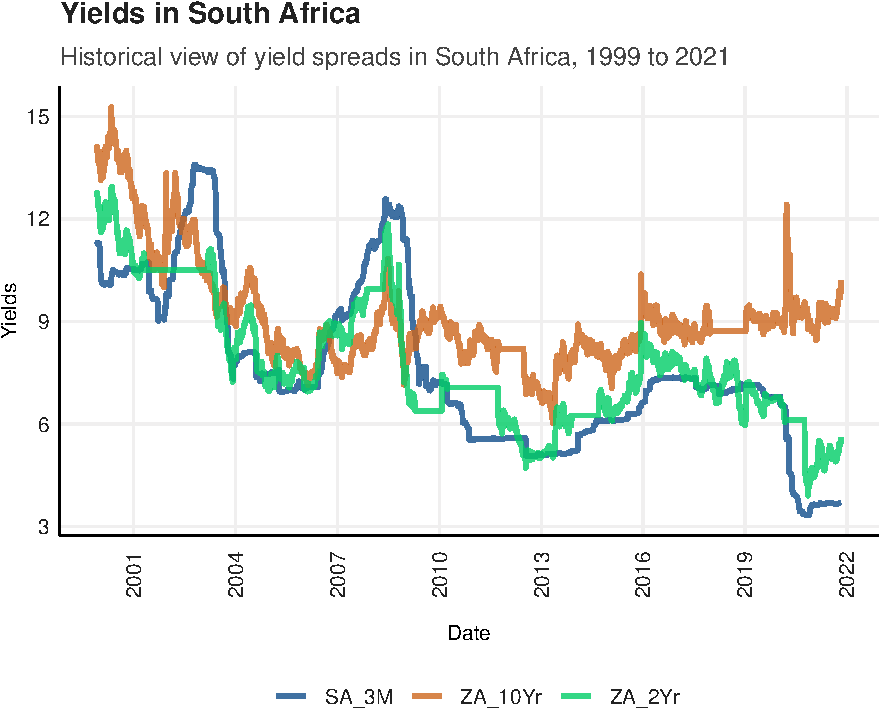
\includegraphics{Question_1_files/figure-latex/unnamed-chunk-1-1.pdf}

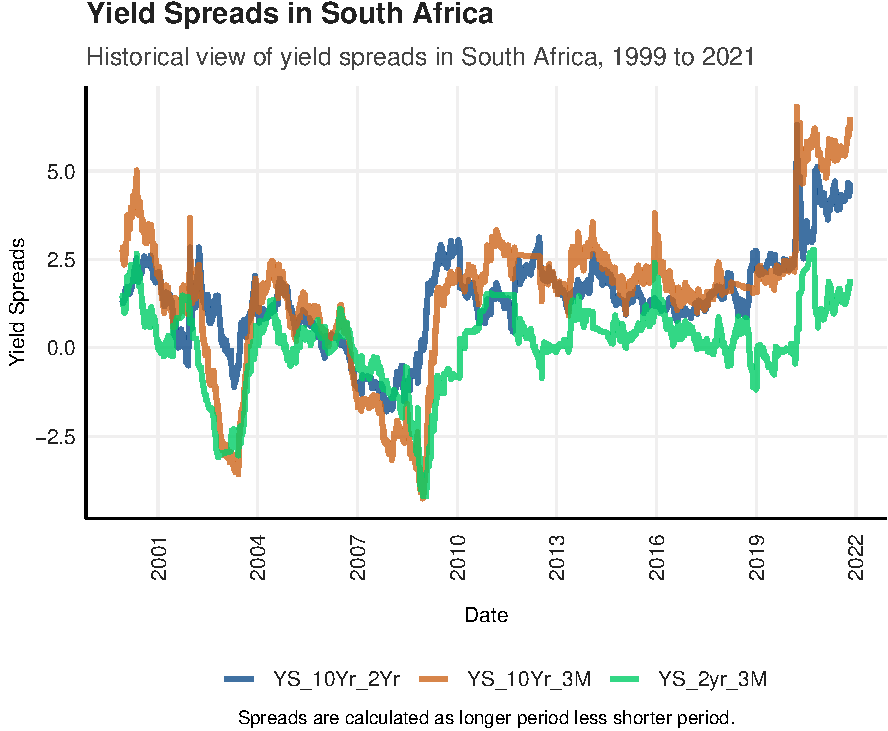
\includegraphics{Question_1_files/figure-latex/unnamed-chunk-2-1.pdf}

\hypertarget{international-sentiment}{%
\section{International Sentiment}\label{international-sentiment}}

Firstly, I plot the USD/ZAR exchange rate to obtain an idea of
volatility in carry trade and capital outflows. This figure shows a
large spike in the exchange rate to levels above R18 per dollar. This is
an indication of substantial capital outlflow out of South Africa. This
is anecdotal evidence to expect that demand for SA bonds decreased
largely by international investors. I argue that the reason we do not
observe this as in the 3-month or 2-year is because of the substantial
SARB intervention.

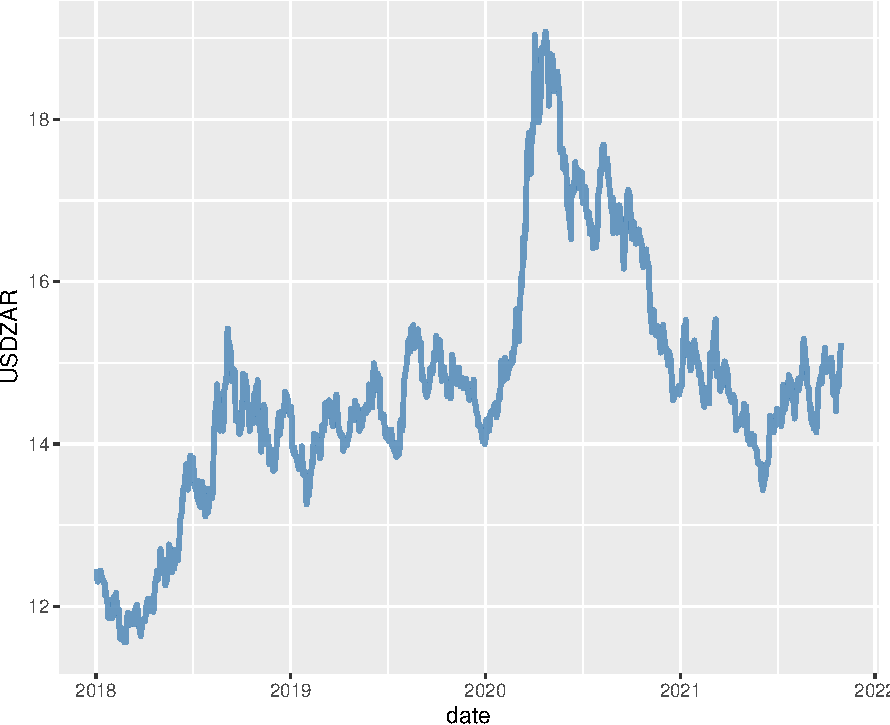
\includegraphics{Question_1_files/figure-latex/unnamed-chunk-3-1.pdf}

To confirm this finding, I compare the yield spread between the SA and
US 10-year bonds, and the yield spread between the SA and US 2-year
bonds. Fedderke (2021) argue that higher South African economic growth,
lower inflation, public and private debt, as well as Rand-Dollar
appreciation are all associated with a statistically significantly lower
South African - United States yield spread. In addition to that, I would
add global risk sentiment as contributing to yield spread evolution
between SA and the US.

The figure shows a clear spike in the yield spread between the US and
SA. The spread is calculated as the SA yield less the US yield. This
confirms that global risk sentiment, movement out of emerging market
bonds and into safer developed markets bond is a contributing factor to
higher yields in South Africa. In addition to this, I have omitted an
discussion of an important factor being inflation. Investors are
concerned about real yields, and therefore, if inflation expectations
increase, then investors demand higher nominal yields to ensure constant
real yields. Initially, there was a fear of deflation in the US, but
this fear became less apparent as fiscal and monetary policy makers
adopted great expansionary policy.

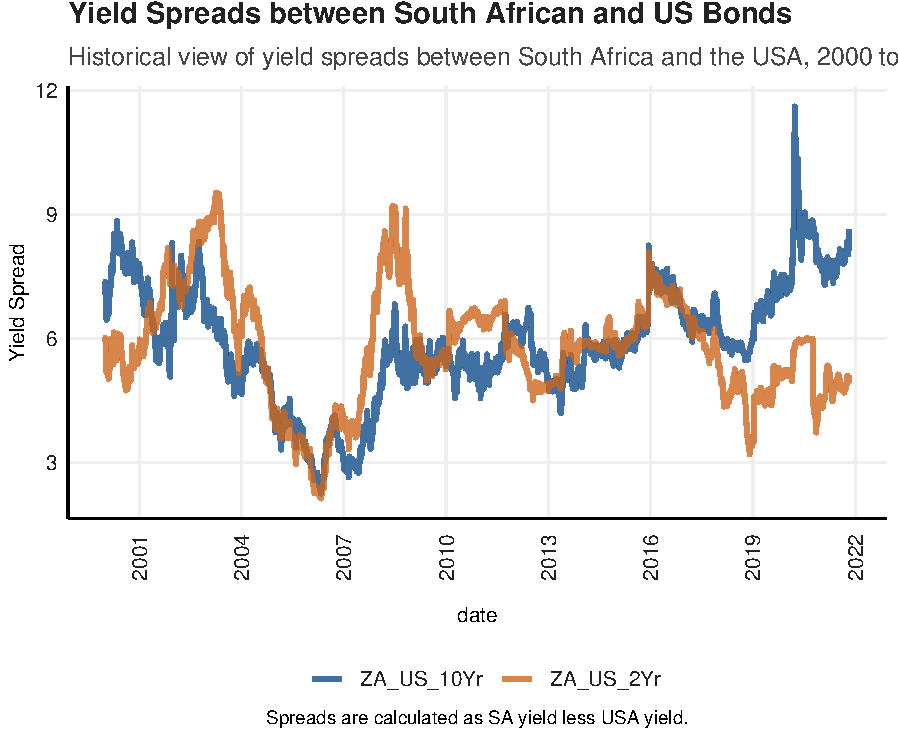
\includegraphics{Question_1_files/figure-latex/unnamed-chunk-4-1.pdf}

\hypertarget{conclusion}{%
\section{Conclusion}\label{conclusion}}

My main line of argument is that capital outflows into safer developed
market bonds caused the demand for South African bonds to decrease, and
therefore their yields to increase. I argue that the substantial action
by the SARB, especially its adoption of a mild form quantative easing
for the first time, kept the 3-month and 2-year yields low. However, the
10-year yield increased, and in turn its spread with bonds of shorter
maturity. Higher yields for expected for longer-term bonds, but I do
agree with the initial hypothesis that the yield spreads are greater
than historical norms.

\newpage

\hypertarget{references}{%
\section*{References}\label{references}}
\addcontentsline{toc}{section}{References}

Fedderke, J.W., 2021. The South African--United States sovereign bond
spread and its association with macroeconomic fundamentals. South
African Journal of Economics.

\hypertarget{appendix}{%
\section*{Appendix}\label{appendix}}
\addcontentsline{toc}{section}{Appendix}

\hypertarget{appendix-a}{%
\subsection*{Appendix A}\label{appendix-a}}
\addcontentsline{toc}{subsection}{Appendix A}

Some appendix information here

\bibliography{Tex/ref}





\end{document}
